\documentclass[ 12 pt]{article}
\usepackage{caption}
%\usepackage{subfig}
\usepackage{csquotes}
\usepackage{natbib}
\usepackage{booktabs}
\usepackage{tabularx}
\usepackage{graphicx}
\usepackage{subcaption}
\usepackage[table]{xcolor}
\usepackage{pdflscape}
\usepackage{longtable}
\usepackage{caption}
\usepackage{threeparttable} 
\usepackage{multirow}
\usepackage{dcolumn} % Align on the decimal point of numbers in tabular columns
\newcolumntype{d}[1]{D{.}{.}{#1}}
\usepackage{threeparttable} % For better formatting of table notes
\setlength{\parindent}{0pt}
\usepackage[top=1in, bottom=0.8in, left=1in, right=1in]{geometry}
\renewcommand*{\arraystretch}{0.8}

\makeatletter
\renewenvironment{table}%
{\renewcommand\familydefault\sfdefault
	\@float{table}}
{\end@float}
\makeatother

\makeatletter
\renewenvironment{figure}%
{\renewcommand\familydefault\sfdefault
	\@float{figure}}
{\end@float}
\makeatother

\usepackage{titlesec}
\titleformat{\section}
{\normalfont\sffamily\Large\bfseries}
{\thesection}{1em}{}
\titleformat{\subsection}
{\normalfont\sffamily\large\bfseries}
{\thesubsection}{1em}{}

\AtBeginEnvironment{tabular}{\sffamily}
\usepackage{arydshln}

\usepackage{etoolbox}
\makeatletter
\patchcmd{\@footnotetext}{\footnotesize}{\footnotesize\sffamily}{}{}
\makeatother

\title{Results of RCT on “Mundus More Math” High Dosage Tutoring program conducted at Mundus College \\ \Large Sept 2017 \-- February 2018}

\author{Prof. Dr. Mario A. Maggioni (UCSC), Dr. Domenico Rossignoli (UCSC), \\ Dr. Joppe de Ree (EUR), D. Walentek (UvA) \\ and Dr. B. Paulle (Principal Investigator, UvA)}

\begin{document}

\sffamily
\maketitle

\section{Introduction}
This research note describes the analysis of the outcome of a High-Dosage Math Tutoring program (HDT) named \enquote{Mundus More Math} or \enquote{M\textsuperscript{3}} (the treatment) applied to an experimental sample at Mundus College (Amsterdam). The goal of the research is to assess the effectiveness of the M\textsuperscript{3} program in improving math skills of the students participating to the research, as compared to a control group who has not been administered any treatment. Further, the research also investigates whether the socio-emotional learning (SEL) component provided within M\textsuperscript{3} program affects some targeted prosocial attitudes and behaviors of the treated students, providing preliminary findings.

The research involved 7 classes belonging to 4 different 8-grade school programs provided at Mundus College in Amsterdam, namely: VMBO-A, VMBO-B, PRO and ISK. The four school programs target different student populations, in term of entry skills and abilities, therefore the impact of heterogeneity on the treatment effect is also taken into account.

\section{Program description: Mundus More Math (M\textsuperscript{3})}
\label{sec:program}
The Bridge Learning Interventions’ (TBLI) is a non-profit, charitable organization dedicated to helping disadvantaged students and their caregivers. SAGA Innovations in the USA developed High Dosage (Math) Tutoring (HDT) and partners with TBLI. The program, or treatment, is TBLI’s first implementation of HDT, complimented by TBLI’s evolving Social Emotional Learning (SEL) program. This represents the first time HDT has ever been attempted at the secondary level outside the US. In September 2017, one hundred first year students entering Mundus College in Amsterdam West were randomly assigned to either Treatment or Control groups. Mundus College serves roughly the most at risk and lowest performing population of any secondary school in Amsterdam (or indeed in the Netherlands). 
So TBLI’s main tool is \enquote{high dosage} tutoring – in this case in the domain of math. During regular school hours, in groups of two, treatment students received one class period (50 minutes) every day of personalized math instruction from \enquote{their own} durably-matched professional tutor. Tutors maintained contact with parents, mostly through phone calls, every week. 

Although HDT normally lasts for an entire schoolyear, due to budgetary constraints, in this case TBLI was forced to experiment with less than \enquote{half dosage}, that is, slightly less than a half a year (September ‘17 to January ’18) of treatment. 
Strong and durable relationships are at the core of everything TBLI does. Tutors build and maintain strong ties with students and their parents; the \enquote{site director} (program manager) maintains strong ties with the teachers and school administration. Implicitly, HDT is always already both a cognitive and a social emotional learning intervention. HDT is designed to augment growth mindsets, (self and collective) efficacy, and emotional and life skills. However, TBLI extends and makes explicit its own SEL component. For example, every tutoring session begins, for all tutors and tutees, with a brief guided meditation framed as a \enquote{concentration practice}. Albeit during only a few hours throughout this initial five month intervention period, on top of this mediation-based SEL approach, TBLI began facilitating it’s own evidence-based SEL program, \enquote{Compass}.  

\section{Data and methods}
A total of 7 classes, belonging to four different school program types at the Mundus College in Amsterdam have been selected for participating into \enquote{M\textsuperscript{3}}, to be evaluated through a rigorous randomized controlled trial procedure. Parents were asked to sign a consent form allowing students to be assigned to either treatment or control groups, and for his/her test scores to be analysed in an anonymous way by the research team.
Once the parents of the target classes have been asked for written and explicit consent to let their children participate to the research, randomization has been implemented. As Table \ref{tab:sample} shows, 98 students provided written consent\footnote{The total number of students invited, as can be inferred from Table \ref{tab:sample} is 110, but 12 students did not produce parents' consent and therefore were not included in the research.} and were randomly assigned to Treatment or Control group through a randomization based on program type, classes and baseline (September 2017) scores in TOA Math Non Verbal\footnote{The TOA is the web-based standardized achievement test Mundus College usually administers.}, according to the following procedure:
\begin{itemize}
	\item firstly, students were ranked according to their baseline score in TOA Math (Non Verbal), i.e. after taking the test in September 2017;
	\item within each class, students were matched in couplets according to their scores; within each couplet, one student was randomly assigned to Treatment, while the other was assigned to Control group.
\end{itemize}

Please note that with regard to the program types (VMBO-A, VMBO-B, ISK and PRO) we stick with the labels provided by the intervention school. To outsiders this may be confusing because VMBO-B might be associated with the track \enquote{basis-beroeps [basic]}. As the following makes clear, this is not the case here. In this case, VMBO-A refers to \enquote{basis-beroeps [basic]}, the lowest vocational trajectory. VMBO-B refers to a mix of \enquote{basis-beroeps [basic]}, \enquote{basis-beroeps/kader [basic/middle]}, the middle vocational trajectory and \enquote{theoretisch [theoretical]}, the highest vocational track. ISK refers to \enquote{Eerste Opvang Anderstaligen [Dutch as Second Language]}, which is also part of \enquote{VMBO basis-beroeps [basic]}. PRO refers to \enquote{Praktijkonderwijs [practical education]} which is best seen as a track in between special education and the lowest vocational track.

Data analysis required each student to attend both test sessions (September 2017, the \enquote{baseline} and February 2018, the \enquote{follow-up}) and a \enquote{treated} case to be \enquote{paired} with a control one. This explains why, starting form an initial sample of 98 students, once dropouts are taken into account, the final sample accrues to 45 students assigned to treatment and 46 assigned to control group.

Table \ref{tab:compliance} illustrates the actual availability of TOA test scores (both versions) compliance. In fact, due to contingent reasons (absence of some students), not all students involved in the research have been able to perform the TOA tests, either in the first (September 2017) or second (February 2018) session. The lack of full compliance generates imbalances in the pairing between treated and control, since there are some treated-control couplets in which either the treated or control student missed at least the September or the February session of the test: in such a case, the pair becomes incomplete. Therefore, since the randomization process is based on the above-mentioned pairing process, all incomplete pairs have been excluded from the analysis\footnote{This deletion has been made \enquote{test-wise}, i.e. specifically for each one of the three TOA tests included in the analysis (Math Non-Verbal, Math Verbal and Reading).}. For this reason, the actual sample of our analysis is limited to a maximum of 76 students for TOA Math (Verbal), to a maximum of 84 students for TOA Math (Non-Verbal) and to a maximum of 72 for TOA Reading test.

This procedure ensures that treated and control samples are always balanced. However, in Section \ref{sec:robustness} we tested whether attrition, both from dropout and non compliance, is random by running the same analysis on the unbalanced samples, finding non substantial differences in effect sizes and significance.

% Table generated by Excel2LaTeX from sheet 'sample'
  \begin{table}[htbp]
  \centering
  \caption{Research sample}
    \begin{tabular}{p{0.5cm}rrrrrrrr}
    \toprule
          &       \multicolumn{2}{r}{No consent} & \multicolumn{6}{c}{Consent} \\ \cmidrule(r){3-3} \cmidrule(r){4-9} 
          &       &       & \multicolumn{3}{c}{Assigned to Treatment} & \multicolumn{3}{c}{Assigned to Control} \\
\cmidrule(r){4-6} \cmidrule(r){7-9}    \multicolumn{1}{c}{\multirow{2}[2]{*}{Program type}} &       &       &       &       & \textbf{Actual} &       &       & \textbf{Actual} \\
          & \multicolumn{1}{l}{Class} &       & \multicolumn{1}{l}{Rand.} & \multicolumn{1}{l}{Dropout} & \textbf{Treated} & \multicolumn{1}{l}{Rand.} & \multicolumn{1}{l}{Dropout} & \textbf{Control} \\
    \midrule
    \multicolumn{1}{c}{\multirow{2}[1]{*}{VMBO-A}} & 1A1   & 2     & 8     &       & \textbf{8} & 8     &       & \textbf{8} \\
          & 1A2   & 2     & 7     & 1     & \textbf{6} & 8     & 1     & \textbf{7} \\  \midrule
    \multicolumn{1}{c}{VMBO-B} & 1B1   & 4     & 8     & 1     & \textbf{7} & 8     & 1     & \textbf{7} \\   \midrule
    \multicolumn{1}{c}{ISK} & 1J1   &       & 9     & 1     & \textbf{8} & 9     &       & \textbf{9} \\   \midrule
    \multicolumn{1}{c}{\multirow{3}[1]{*}{PRO}} & 1R2   & 1     & 5     &       & \textbf{5} & 6     &       & \textbf{6} \\
          & 1R3   & 3     & 5     & 1     & \textbf{4} & 5     & 1     & \textbf{4} \\
          & 1R4   &       & 6     &       & \textbf{6} & 6     &       & \textbf{6} \\
    \midrule
    Total &       & 12    & 49    & 4     & \textbf{45} & 49    & 3     & \textbf{46} \\
    \bottomrule
    \end{tabular}%
  \label{tab:sample}%
\end{table}%
%% Table generated by Excel2LaTeX from sheet 'Foglio1'
\begin{table}[htbp]
  \centering
  \caption{Add caption}
    \begin{tabular}{l|rrrr|rrrr}
    \toprule
          & \multicolumn{4}{c|}{TOA Math Non-Verbal} & \multicolumn{4}{c}{TOA Math} \\
          & \multicolumn{2}{c}{Treated} & \multicolumn{2}{c|}{Control} & \multicolumn{2}{c}{Treated} & \multicolumn{2}{c}{Control} \\
    Class & \multicolumn{1}{l}{Non compliant} & Compliant & \multicolumn{1}{l}{Non compliant} & Compliant & \multicolumn{1}{l}{Non compliant} & Compliant & \multicolumn{1}{l}{Non compliant} & Compliant \\
    \midrule
    1A1   & 1     & 7     & 0     & 8     & 0     & 8     & 1     & 7 \\
    1A2   & 0     & 7     & 0     & 7     & 2     & 5     & 3     & 4 \\
    1B1   & 0     & 7     & 0     & 7     & 0     & 7     & 0     & 7 \\
    1J1   & 1     & 7     & 1     & 8     & 0     & 8     & 1     & 8 \\
    1R2   & 0     & 6     & 0     & 6     & 2     & 4     & 1     & 5 \\
    1R3   & 0     & 4     & 0     & 4     & 0     & 4     & 0     & 4 \\
    1R4   & 0     & 6     & 1     & 5     & 0     & 6     & 0     & 6 \\
    Total & 2     & 44    & 2     & 45    & 4     & 42    & 6     & 41 \\
    \bottomrule
    \end{tabular}%
  \label{tab:addlabel}%
\end{table}%


% Table generated by Excel2LaTeX from sheet 'data availability'
\begin{table}[htbp]
  \centering
  \caption{Compliance for TOA Math tests}
    \begin{tabular}{lllllllll}
    \toprule
          & \multicolumn{4}{c}{TOA Math Non-Verbal} & \multicolumn{4}{c}{TOA Math} \\ \cmidrule(r){2-5} \cmidrule(r){6-9}
          & \multicolumn{2}{c}{Treated} & \multicolumn{2}{c}{Control} & \multicolumn{2}{c}{Treated} & \multicolumn{2}{c}{Control} \\ \cmidrule(r){2-3} \cmidrule(r){4-5} \cmidrule(r){6-7} \cmidrule(r){8-9}
    Class & \multicolumn{1}{c}{NC} & \multicolumn{1}{c}{C} & \multicolumn{1}{c}{NC} & \multicolumn{1}{c}{C} & \multicolumn{1}{c}{NC} & \multicolumn{1}{c}{C} & \multicolumn{1}{c}{NC} & \multicolumn{1}{c}{C} \\
    \midrule
    1A1   & \multicolumn{1}{c}{1} & \multicolumn{1}{c}{7} & \multicolumn{1}{c}{0} & \multicolumn{1}{c}{8} & \multicolumn{1}{c}{0} & \multicolumn{1}{c}{8} & \multicolumn{1}{c}{1} & \multicolumn{1}{c}{7} \\
    1A2   & \multicolumn{1}{c}{0} & \multicolumn{1}{c}{7} & \multicolumn{1}{c}{0} & \multicolumn{1}{c}{7} & \multicolumn{1}{c}{2} & \multicolumn{1}{c}{5} & \multicolumn{1}{c}{3} & \multicolumn{1}{c}{4} \\
    1B1   & \multicolumn{1}{c}{0} & \multicolumn{1}{c}{7} & \multicolumn{1}{c}{0} & \multicolumn{1}{c}{7} & \multicolumn{1}{c}{0} & \multicolumn{1}{c}{7} & \multicolumn{1}{c}{0} & \multicolumn{1}{c}{7} \\
    1J1   & \multicolumn{1}{c}{1} & \multicolumn{1}{c}{7} & \multicolumn{1}{c}{1} & \multicolumn{1}{c}{8} & \multicolumn{1}{c}{0} & \multicolumn{1}{c}{8} & \multicolumn{1}{c}{1} & \multicolumn{1}{c}{8} \\
    1R2   & \multicolumn{1}{c}{1} & \multicolumn{1}{c}{5} & \multicolumn{1}{c}{0} & \multicolumn{1}{c}{6} & \multicolumn{1}{c}{3} & \multicolumn{1}{c}{3} & \multicolumn{1}{c}{1} & \multicolumn{1}{c}{5} \\
    1R3   & \multicolumn{1}{c}{0} & \multicolumn{1}{c}{4} & \multicolumn{1}{c}{0} & \multicolumn{1}{c}{4} & \multicolumn{1}{c}{0} & \multicolumn{1}{c}{4} & \multicolumn{1}{c}{0} & \multicolumn{1}{c}{4} \\
    1R4   & \multicolumn{1}{c}{0} & \multicolumn{1}{c}{6} & \multicolumn{1}{c}{1} & \multicolumn{1}{c}{5} & \multicolumn{1}{c}{0} & \multicolumn{1}{c}{6} & \multicolumn{1}{c}{0} & \multicolumn{1}{c}{6} \\ \midrule
    Total & \multicolumn{1}{c}{3} & \multicolumn{1}{c}{43} & \multicolumn{1}{c}{2} & \multicolumn{1}{c}{45} & \multicolumn{1}{c}{5} & \multicolumn{1}{c}{41} & \multicolumn{1}{c}{6} & \multicolumn{1}{c}{41} \\
    \midrule
    \multicolumn{9}{l}{NC = Non Compliant; C= Compliant} \\
    \end{tabular}%
  \label{tab:compliance}%
\end{table}%

% \input{TOA-NV-compliance.tex}
% \input{TOA-compliance.tex}

The analysis investigates two potential effects of M\textsuperscript{3}: improving math skills, through the core component of the 1-to-2 high dosage tutoring, and improving prosocial behaviour and attitudes, through the Socio-Emotional Learning component.
In order to test the effect of the treatment on math skills, we focused on the outcome of two standard test scores, widely adopted nationwide in the Netherlands to assess the school performance of students, namely the Verbal and Non-Verbal versions of the Math tests provide by TOA. Since our sample includes also students from international program (ISK) as well as students with family background that could affect their language skills in Dutch, our main focus is on the Non-Verbal version of the test, which is specifically designed to assess math skills independently of language ability, i.e. purging the test from possible biases arising from lack of comprehension of the textual instructions, rather only targeting math skills. Further, in order to exclude potential unintended negative side-effects on non-math related skills (since M\textsuperscript{3} could skew students' efforts away from learning non-math related subjects) we also tested whether M\textsuperscript{3} affects the outcome of a Reading score, provided again by TOA. Therefore, the analysis focuses on the following three dependent variables:
\begin{itemize}
\item TOA Math (Non-Verbal)
\item TOA Math (Verbal)
\item TOA Reading
\end{itemize}

All three tests were first taken in September 2017 (baseline), before random assignment to the program started, and then in February 2018 (follow-up), after the end of M\textsuperscript{3}. Table \ref{tab:sum_by_wave_paired} shows the summary statistics of the three tests, by treatment group and test session.

In order to increase cross-test and cross-study comparability, all test scores have been standardized as follows:

\begin{displaymath}
z_{i}=\frac{x_{i}-\overline{x_{C}}}{\sigma_{C}}
\end{displaymath}

where $z_{i}$ is the standardized value of the test score for student $i$, $x_{i}$ is the raw value of the test score for student $i$, $\overline{x_{C}}$ is the mean value of the test score in the Control group and $\sigma_{C}$ is the standard deviation of the test score for the Control group. This standardization is \enquote{anchored} to the Control group performance, i.e. to the attendance of regular classes in absence of treatment.

Therefore, all treatment effects in Section \ref{sec:results} are presented in this standardized form.  

The effect of the treatment has been estimated through OLS regressions, including pairs fixed-effects (FE), to account for idiosyncratic characteristics of students within each pair, and robust standard errors, to correct for potential heteroskedasticity. As an additional check, we alternatively accounted for possible class-specific effects by including class FE. Finally, the same models have been estimated by including the baseline outcome of the dependent variable, namely the outcome of the math test taken in September 2017, to account for possible ex-ante differences in math skills. 

\section{Results}
\label{sec:results}
\subsection{Effect on math skills (TOA Math Non Verbal and Verbal)}
Figure \ref{fig:hists} outlines the main outcome of the analysis: the distributions of the differences between February 2018 and September 2017 TOA scores is shifted to the right for Treated, indicating that students enrolled in M\textsuperscript{3} performed generally better than their control peers in both the Non-Verbal (left panel) and Verbal (right panel) TOA Math tests. This outcome seems particularly more evident for the Non-Verbal version of the test, which is the main target of our research. On average, after 5 months of M\textsuperscript{3}, the treated group increased math TOA score by 8.9 points in the Non-Verbal version (max 50 points) and by 9.6 points in the Verbal version (max 54 points).
The same outcome can be observed in the last column of Table \ref{tab:sum_by_wave_paired}, that shows that a positive and significant difference for both math tests is present in both treated and control group (thus identifying a positive effect of attending regular math lessons at school), although it is larger and highly significant for the treated, as compared to the counter-factual control group.

\begin{figure}[!h]
\caption{Distribution of differences in TOA scores (September vs February)}
\begin{subfigure}{.5\textwidth}
  \centering
	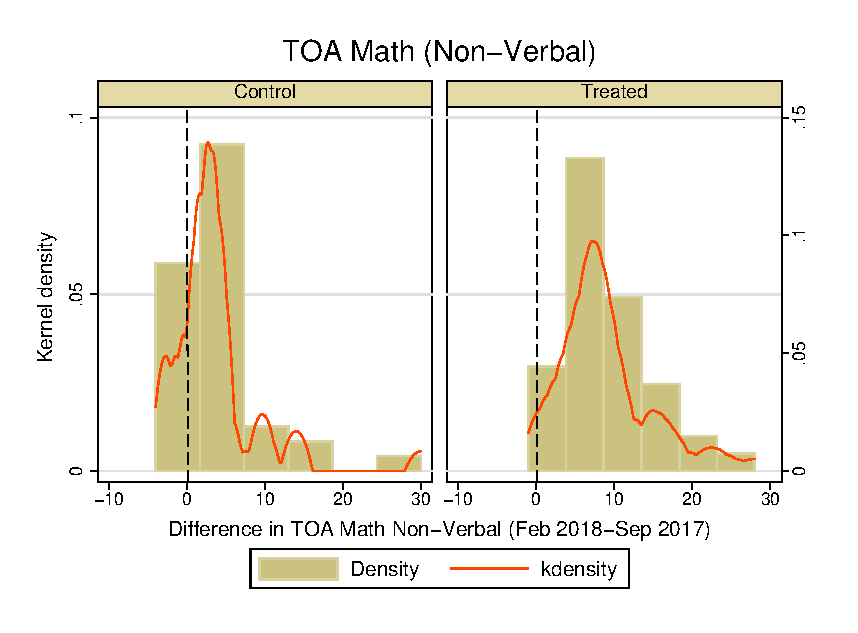
\includegraphics[width=.8\linewidth]{HIST_MATH_NON_VERB.eps}
  \caption{TOA Math (Non-Verbal)}
  \label{fig:histNV}
\end{subfigure}%
\begin{subfigure}{.5\textwidth}
  \centering
  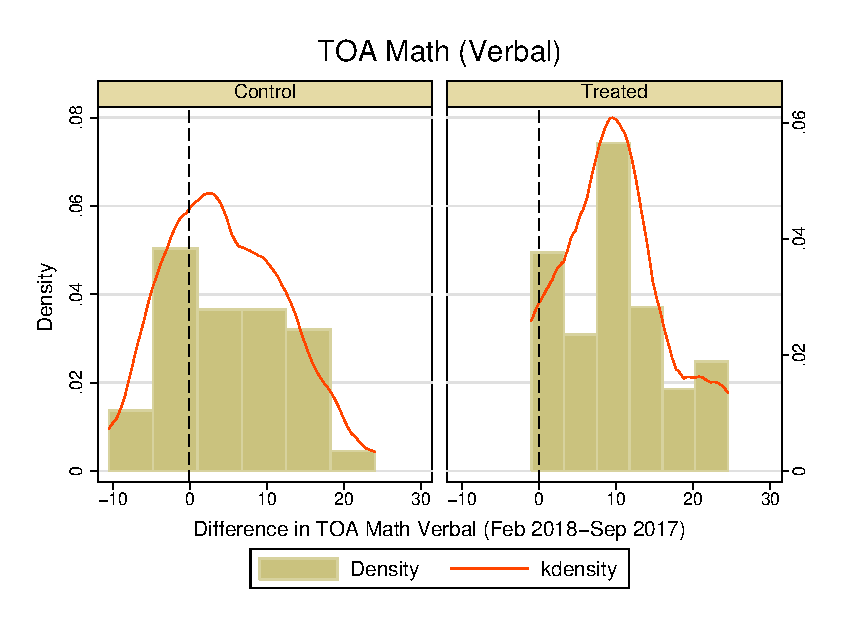
\includegraphics[width=.8\linewidth]{HIST_MATH_VERB.eps}
  \caption{TOA Math (Verbal)}
	\label{fig:histVERB}
\end{subfigure}
\label{fig:hists}
\end{figure}

% Table generated by Excel2LaTeX from sheet 'Foglio1'
\begin{table}[htbp]
  \centering
  \caption{Summary of TOA test scores, by wave and treatment group}
    \begin{tabular}{lrrrrrrrr}
    \toprule
          & \multicolumn{3}{c}{September 2017} & \multicolumn{3}{c}{February 2018} &       & \\\cmidrule(lr){2-4}\cmidrule(lr){5-7}
    Test score & \multicolumn{1}{l}{Obs} & \multicolumn{1}{l}{Mean} & \multicolumn{1}{l}{SD} & \multicolumn{1}{l}{Obs} & \multicolumn{1}{l}{Mean} & \multicolumn{1}{l}{SD} & Diff & Sig \\
    \midrule
    \multicolumn{1}{l}{\textit{Treated}} &       &       &       &       &       &       &       &  \\
    TOA Math (Non-Verbal) & 42    & 20.17 & 8.59  & 42    & 29.07 & 8.62  & 8.90  & *** \\
    TOA Math (Verbal) & 38    & 22.67 & 2.08  & 38    & 32.29 & 11.21 & 9.62  & *** \\
    TOA Reading & 36    & 28.08 & 8.73  & 36    & 28.78 & 6.93  & 1.86  & NS \\
    \multicolumn{1}{l}{\textit{Control}} &       &       &       &       &       &       &       &  \\
    TOA Math (Non-Verbal) & 42    & 19.71 & 8.90  & 42    & 23.19 & 8.57  & 3.48  & * \\
    TOA Math (Verbal) & 38    & 22.37 & 13.18 & 38    & 26.92 & 9.68  & 4.55  & * \\
    TOA Reading & 36    & 28.14 & 6.63  & 36    & 28.31 & 6.98  & 0.17  & NS \\
    \bottomrule
    \multicolumn{9}{l}{\footnotesize Tests performed on full compliant pairs only.}\\
\multicolumn{9}{l}{\footnotesize * p$<$0.10, ** p$<$0.05, *** p$<$0.01}\\
    \end{tabular}%
  \label{tab:sum_by_wave_paired}%
\end{table}%


The econometric results of the analysis confirm and strengthen the hints arising from descriptive statistics. 
Table \ref{tab:toarekNV} shows the standardized results for the Non-Verbal version of the TOA test and Table \ref{tab:toarek} for the Verbal version of the TOA Math test. Both tables show that the effect of M\textsuperscript{3} is always strongly positive and significant and robust to controlling for the randomization's pairs (i.e. a measure of \enquote{student types}), students' classes and baseline outcomes (i.e. score of the same test in September 2017, before randomization took place). Notably, the effect ranges between 0.66 and 0.68 of a standard deviation for the Non Verbal version of the TOA Math test, and between 0.54 to 0.56 for the Verbal version. This result is strong compared to established evidence in the literature and it is also encouraging since the best result is obtained in the Non-Verbal version of the math test, that does not penalize students that improved in math despite their language disadvantages.

\begin{table}[htbp]\centering
\def\sym#1{\ifmmode^{#1}\else\(^{#1}\)\fi}
\caption{TOA Math (Non-language): Treatment effect, OLS}
\begin{tabular}{l*{4}{D{.}{.}{-1}}}
\toprule
                    &\multicolumn{2}{c}{Benchmark models}           &\multicolumn{2}{c}{Including baseline outcome} \\\cmidrule(lr){2-3}\cmidrule(lr){4-5}
                    &\multicolumn{1}{c}{(1)}   &\multicolumn{1}{c}{(2)}   &\multicolumn{1}{c}{(3)}   &\multicolumn{1}{c}{(4)}   \\
\midrule
Treatment effect    &               0.686***&               0.686***&               0.676***&               0.658***\\
                    &             (0.118)   &             (0.164)   &             (0.115)   &             (0.127)   \\
Baseline outcome	&                       &                       &               0.208   &               0.563***\\
                    &                       &                       &             (0.184)   &             (0.112)   \\
Pair FE             &                 Yes   &                  No   &                 Yes   &                  No   \\
Class FE            &                  No   &                 Yes   &                  No   &                 Yes   \\
\midrule
Obs                 &                  84   &                  84   &                  84   &                  84   \\
LL                  &                 -37   &                 -91   &                 -35   &                 -69   \\
AIC                 &                 160   &                 198   &                 159   &                 157   \\
BIC                 &                 265   &                 218   &                 266   &                 179   \\
\bottomrule
\multicolumn{5}{l}{\footnotesize Standardized coefficients; Robust standard errors in parentheses}\\
\multicolumn{5}{l}{\footnotesize Dependent variable: test score in Feb 2018; Baseline outcome: test score in Sept 2017.}\\
\multicolumn{5}{l}{\footnotesize * p$<$0.10, ** p$<$0.05, *** p$<$0.01}\\
\end{tabular}
\label{tab:toarekNV}
\end{table} 
\begin{table}[htbp]\centering
\def\sym#1{\ifmmode^{#1}\else\(^{#1}\)\fi}
\caption{TOA Math (Verbal): Treatment effect, OLS}
\begin{tabular}{l*{4}{D{.}{.}{-1}}}
\toprule
                    &\multicolumn{2}{c}{Benchmark models}           &\multicolumn{2}{c}{Including baseline outcome} \\\cmidrule(lr){2-3}\cmidrule(lr){4-5}
                    &\multicolumn{1}{c}{(1)}   &\multicolumn{1}{c}{(2)}   &\multicolumn{1}{c}{(3)}   &\multicolumn{1}{c}{(4)}   \\
\midrule
Treatment effect         &               0.555***&               0.555***&               0.545***&               0.537***\\
                    &             (0.130)   &             (0.167)   &             (0.124)   &             (0.137)   \\
Baseline outcome     &                       &                       &               0.413*  &               0.787***\\
                    &                       &                       &             (0.219)   &             (0.120)   \\
Pair FE             &                 Yes   &                  No   &                 Yes   &                  No   \\
Class FE            &                  No   &                 Yes   &                  No   &                 Yes   \\
\midrule
Obs                 &                  76   &                  76   &                  76   &                  76   \\
LL                  &                 -37   &                 -80   &                 -33   &                 -64   \\
AIC                 &                 152   &                 175   &                 147   &                 145   \\
BIC                 &                 243   &                 194   &                 240   &                 166   \\
\bottomrule
\multicolumn{5}{l}{\footnotesize Standardized coefficients; Robust standard errors in parentheses}\\
\multicolumn{5}{l}{\footnotesize Dependent variable: test score in Feb 2018; Baseline outcome: test score in Sept 2017.}\\
\multicolumn{5}{l}{\footnotesize * p$<$0.10, ** p$<$0.05, *** p$<$0.01}\\
\end{tabular}
\label{tab:toarek}
\end{table}
 

Figure \ref{fig:bars} provides a clear and perhaps more straightforward picture of the main effects of M\textsuperscript{3} on the treated sample. The bar chart shows the evolution from September 2017 to February 2018 of the average outcome of the TOA Math (Non-Verbal) test by program type, for both treatment and control groups. In panel \ref{fig:barNV}, the dashed line highlights that after 5-months of Mundus More Math M\textsuperscript{3}, treated students in PRO classes have surpassed control VMBO-A students, namely their next-in-ranking peers, who did not participate in the treatment program. The same positive effect is recorded also for ISK students. A smaller, though still positive, effect is recorded also for the Verbal version of the TOA test (see panel \ref{fig:barVERB}. Here the dashed line highlights that a gap is still existing after 5-months of M\textsuperscript{3}, between treated students in PRO classes and control VMBO-A students, although almost half the distance has been closed. Conversely, ISK students confirm the catching-up and leapfrogging shown in panel \ref{fig:barNV}.

\begin{figure}[!h]
\caption{Overview of treatment effect, by school program type)}
\begin{subfigure}{.5\textwidth}
  \centering
	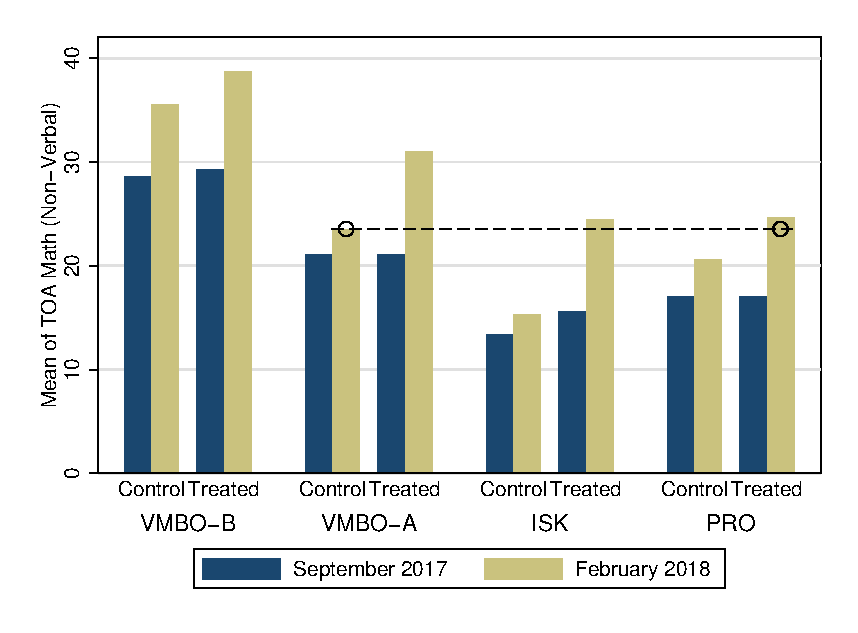
\includegraphics[width=.8\linewidth]{bar_school4_line.eps}
  \caption{TOA Math (Non-Verbal)}
  \label{fig:barNV}
\end{subfigure}%
\begin{subfigure}{.5\textwidth}
  \centering
  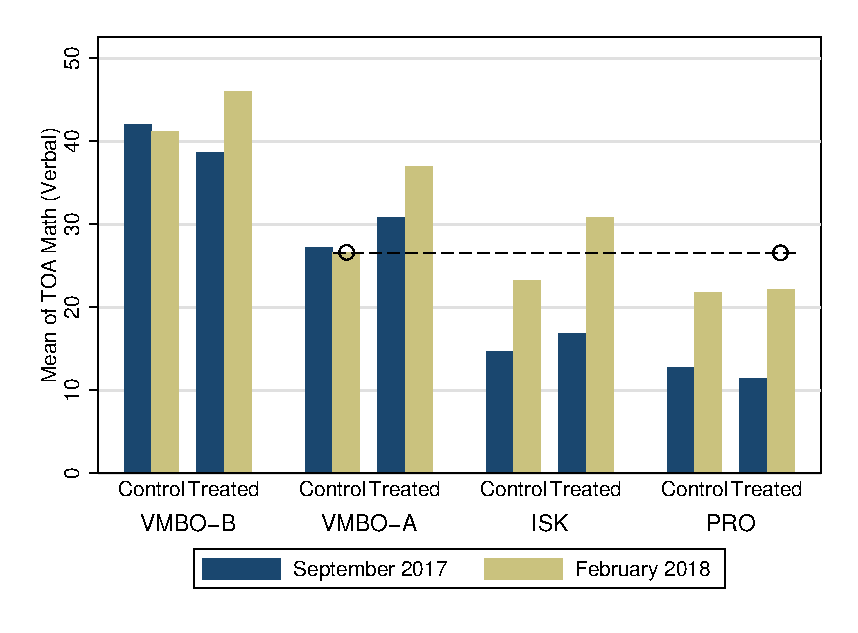
\includegraphics[width=.8\linewidth]{bar_school4_line_VERBAL.eps}
  \caption{TOA Math (Verbal)}
	\label{fig:barVERB}
\end{subfigure}
\label{fig:bars}
\end{figure}

In summary, the main results of our analysis confirm that M\textsuperscript{3} has a significant and strong effect on the treated sample, increasing their math skills abilities, as measured by TOA Math Non Verbal and Verbal tests.

\subsection{Check for unintended negative side-effects}
We also checked for possible unintended negative consequences of high dosage math tutoring in skewing students’ efforts and commitments towards a quantitative subject (math) and away from distinct complementary skills such as reading. To test whether such a negative side-effect occurred in our sample we performed the same analysis shown in Section \ref{sec:results} on the TOA Reading test, taken by the students before (September 2017) and after (February 2018) the treatment program. Results are shown in Table \ref{tab:toalezen}. As the table shows, no negative and significant coefficients is reported, thus excluding any negative side-effect on reading skills for the treated group due to the enrollment in HDT.

\begin{table}[htbp]\centering
\def\sym#1{\ifmmode^{#1}\else\(^{#1}\)\fi}
\caption{Inspecting side-effects of HDT on TOA Reading, OLS}
\begin{tabular}{l*{4}{D{.}{.}{-1}}}
\toprule
                    &\multicolumn{2}{c}{Benchmark models}           &\multicolumn{2}{c}{Including baseline outcome} \\\cmidrule(lr){2-3}\cmidrule(lr){4-5}
                    &\multicolumn{1}{c}{(1)}   &\multicolumn{1}{c}{(2)}   &\multicolumn{1}{c}{(3)}   &\multicolumn{1}{c}{(4)}   \\
\midrule
Treatment effect    &              0.068   &              0.068   &              0.072   &              0.072   \\
                    &             (0.197)   &             (0.195)   &             (0.168)   &             (0.166)   \\
Baseline outcome &                       &                       &               0.451***&               0.476***\\
                    &                       &                       &             (0.122)   &             (0.118)   \\
Pair FE             &                 Yes   &                  No   &                 Yes   &                  No   \\
Class FE            &                  No   &                 Yes   &                  No   &                 Yes   \\
\midrule
Obs                 &                  72   &                  72   &                  72   &                  72   \\
LL                  &                 -63   &                 -84   &                 -51   &                 -72   \\
AIC                 &                 201   &                 184   &                 178   &                 162   \\
BIC                 &                 285   &                 203   &                 264   &                 183   \\
\bottomrule
\multicolumn{5}{l}{\footnotesize Standardized beta coefficients; Standard errors in parentheses}\\
\multicolumn{5}{l}{\footnotesize Dependent variable: test score in Feb 2017; Baseline outcome: test score in Sept 2017.}\\
\multicolumn{5}{l}{\footnotesize * p$<$0.10, ** p$<$0.05, *** p$<$0.01}\\
\end{tabular}
\label{tab:toalezen}
\end{table}


\section{Robustness checks}
\label{sec:robustness}
This section provides a set of robustness checks to the analysis performed above. Sensitivity of the results may arise due to:
\begin{itemize}
\item potential sources of heterogeneity;
\item sampling and balancing issues.
\end{itemize} 

\subsection{Potential sources of heterogeneity}
A potential concern over heterogeneity of M\textsuperscript{3} can arise from the inspection of the models' diagnostics. In particular, to asses the effectiveness of the treatment across different program types, we plotted the residuals of our model against the predicted values, showing a potential concern for clustering of higher levels of test scores for VMBO-B students and lower for PRO students. Figure \ref{fig:rvf_toaNV} and \ref{fig:rvf_toa} shows the usual residual versus fitted scatter plot highlighting in different colors observations belonging to different program types. As both figures show, the highest ranking students enrolled in VMBO program types (green dots in the graph) report systematically larger test score than their peers in both PRO and ISK. 

\begin{figure}[!h]
\begin{subfigure}{.5\textwidth}
  \centering
	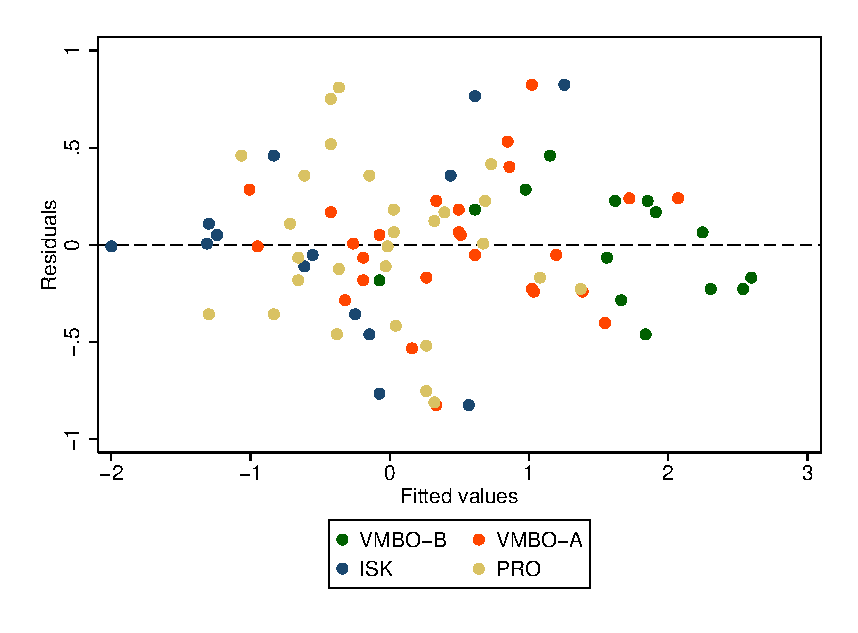
\includegraphics[width=.8\linewidth]{rvfplot_toarekenen_nv2NEW.eps}
  \caption{TOA Math (Non-Verbal)}
  \label{fig:rvf_toaNV}
\end{subfigure}%
\begin{subfigure}{.5\textwidth}
  \centering
  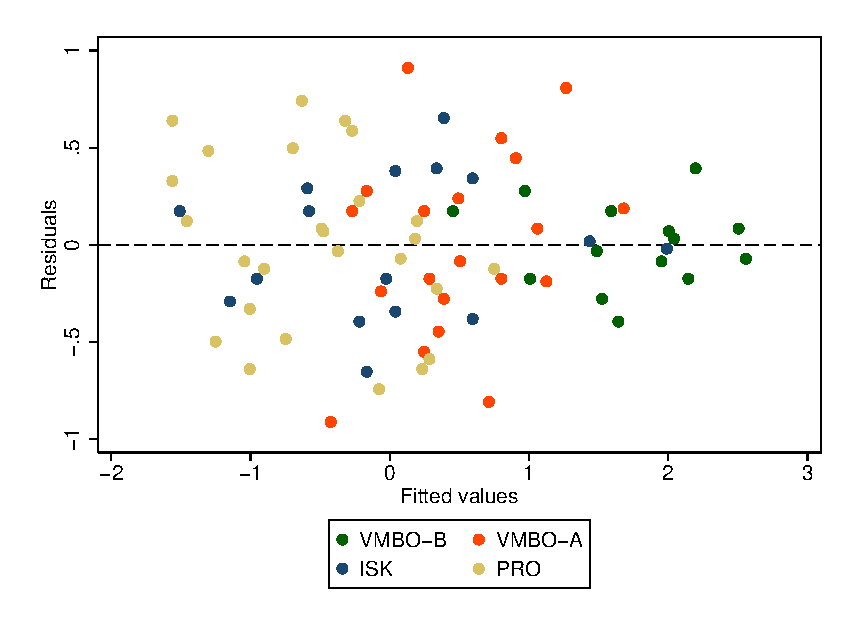
\includegraphics[width=.8\linewidth]{rvfplot_toarekenen2NEW.eps}
  \caption{TOA Math (Verbal)}
	\label{fig:rvf_toa}
\end{subfigure}
\caption{Residual versus fitted plot after estimation in models 1 of Table \ref{tab:toarekNV} (\ref{fig:rvf_toaNV}) and \ref{tab:toarek} (\ref{fig:rvf_toa})}
\label{fig:rvfplots}
\end{figure}

For this reason, we tested whether the strength of the result is unaffected when the different types of school programs by interacting the treatment variable with each program type, using both our benchmark and extended specifications (i.e. those including the baseline test score), as in Tables \ref{tab:toarekNV} and \ref{tab:toarek}).
As table \ref{tab:toaboth} shows, when looking at the Non Verbal version of the TOA Math test, we identify a significant differential effect of program types on the treatment effect, which is stronger for VMBO-A and ISK students as compared to the reference category (VMBO-B, i.e. the highest ranking student program), while it is statistically indistinguishable for PRO students. Therefore, with regard to our main outcome variable, the effect is heterogeneous although heterogeneity does no harm to the most vulnerable students in the sample (PRO), while it generates higher impacts on VMBO-A and ISK. Finally, as columns 3 and 4 show, heterogeneity almost disappears when the outcome variable is TOA Math Verbal. Overall, we find limited heterogeneity in M\textsuperscript{3} effect driven by program type.

\begin{landscape}
\begin{table}[htbp]\centering
\def\sym#1{\ifmmode^{#1}\else\(^{#1}\)\fi}
\caption{TOA performance controlling for program type: Treatment effect, OLS}
\begin{tabular}{l*{4}{D{.}{.}{-1}}}
\toprule
                    &\multicolumn{2}{c}{TOA Math (Non Verbal)}&\multicolumn{2}{c}{TOA Math (Verbal)}               \\\cmidrule(lr){2-3}\cmidrule(lr){4-5}
                    &\multicolumn{1}{c}{(1)}   &\multicolumn{1}{c}{(2)}   &\multicolumn{1}{c}{(3)}   &\multicolumn{1}{c}{(4)}   \\
\midrule
Treatment effect             &               0.367** &               0.351** &               0.502***&               0.564***\\
                    &             (0.160)   &             (0.162)   &             (0.166)   &             (0.188)   \\
Treated $\times$ VMBO-A&               0.508** &               0.524** &               0.573*  &               0.442   \\
&             (0.243)   &             (0.242)   &             (0.311)   &             (0.306)   \\
Treated $\times$ ISK&               0.700*  &               0.670*  &               0.286   &               0.184   \\
&             (0.385)   &             (0.381)   &             (0.298)   &             (0.308)   \\
Treated $\times$ PRO&               0.100   &               0.117   &              -0.462*  &              -0.498*  \\
&             (0.270)   &             (0.272)   &             (0.261)   &             (0.268)   \\
VMBO-A              &              -1.830** &              -1.333   &              -2.714***&              -2.133***\\
                    &             (0.776)   &             (0.887)   &             (0.707)   &             (0.748)   \\
ISK                 &              -1.692** &              -1.377** &              -2.312***&              -1.871***\\
                    &             (0.693)   &             (0.603)   &             (0.588)   &             (0.637)   \\
PRO                 &              -1.275***&              -1.016***&              -2.093***&              -1.513** \\
                    &             (0.183)   &             (0.307)   &             (0.426)   &             (0.665)   \\
Baseline outcome&                       &               0.192   &                       &                 0.245     \\
                    &                       &             (0.133)   &                       &              (0.229)  \\
Pair FE             &                 Yes   &                 Yes   &                 Yes   &                 Yes   \\
\midrule
Obs                 &                  84   &                  84   &                  76   &                  76   \\
LL                  &                 -32   &                 -30   &                 -25   &                 -23   \\
AIC                 &                 154   &                 154   &                 133   &                 132   \\
BIC                 &                 263   &                 268   &                 231   &                 232   \\
\bottomrule
\multicolumn{5}{l}{\footnotesize Standardized coefficients; Robust standard errors in parentheses. Reference category for school type (omitted):}\\
\multicolumn{5}{l}{\footnotesize VMBO-B. Dependent variable: test score in Feb 2018; Baseline outcome: test score in Sept 2017.}\\
\multicolumn{5}{l}{\footnotesize * p$<$0.10, ** p$<$0.05, *** p$<$0.01}\\
\end{tabular}
\label{tab:toaboth} 
\end{table}

\end{landscape}

A further potential source of heterogeneity can arise from differences in tutors’ ability to convey the treatment contents, since the program consists of tight 1-to-2 interactions between tutors and schoolchildren and therefore this relation plays an important role. 
To assess the potential heterogeneity driven by tutors' abilities, we performed the following test. Firstly, we run the same models as in Table \ref{tab:toarekNV} and \ref{tab:toarek}, in which the treatment variable is interacted with each one of the tutors (except one, chosen as reference category), excluding the dummies fixed effect, since the focus now is on the treated\footnote{As a robustness check, we also estimated the same model included Pair FE. The results, as expected are slightly different, since in this case one out of 10 comparisons (tutor 4 with tutor 1) is statistically significant at the 5\% level, and one is weakly significant at 10\%. This difference is likely driven by the fact that each tutor was assigned a small number of students, hence including or excluding a further set of dummy variables in the model (the pair FE) is very likely to affect the composition of the actual available sample and consequently to affect the p-value of each interactive effect, which relies on a very limited number of observations. A similar result is obtained when performing the same pairwise tests for TOA Math Verbal. However, the slightly difference in outcome does not alter the overall picture of a substantially homogeneous effect of M\textsuperscript{3} across tutors.}; then we performed pairwise tests for the interacted terms, in order to compare each tutor's effect with all the other; the outcome of these tests has been summarized in the 5X5 matrix shown in Table \ref{tab:tutormatrix}: only the comparison between Tutors 2 and 3 is significantly different from 0: therefore we can exclude that a systematic difference among tutors' ability biased the treatment effect.

% Table generated by Excel2LaTeX from sheet 'Foglio1'
\begin{table}[htbp]
  \centering
  \renewcommand{\arraystretch}{1.1}
  \caption{Pairwise comparison of Tutor interactive effects (TOA Math Non Verbal)}
\begin{tabular}{p{3cm}p{2.3cm}p{2.3cm}p{2.3cm}p{2.3cm}p{2.3cm}}
    \midrule
          & Tutor\_1 & Tutor\_2 & Tutor\_3 & Tutor\_4 & Tutor\_5 \\
    Tutor\_1 & \cellcolor{black}  &       &       &       &  \\
    Tutor\_2 & NS    & \cellcolor{black}  &       &       &  \\
    Tutor\_3 & NS   & 0.05    & \cellcolor{black}  &       &  \\
    Tutor\_4 & NS    & NS & NS    & \cellcolor{black}  &  \\
    Tutor\_5 & NS    & NS    & NS    & NS    & \cellcolor{black}  \\
    \midrule
    \multicolumn{6}{l}{\footnotesize Reference category: Tutor\_1, the coefficient refers to \enquote{treatment} coefficient.} \\
    \multicolumn{6}{l}{\footnotesize Pairwise tests. Dep. var.: TOA Math Non Verbal (Feb 2018); Regressors: treatment, baseline outcome.} \\
    \end{tabular}%
  \label{tab:tutormatrix}%
\end{table}%


Finally, we further explored possible heterogeneity due to tutors' abilities by assessing the effect of including or excluding class FE from the analysis: in fact, since the assignment of tutors to tutees was not completely random, but driven by organizational reasons, it is likely that different tutors have been assigned different students (in term of average ability). This seems to be the case, since both Tables \ref{tab:tutorNV_class} and \ref{tab:tutor_class} report significant coefficients for the interacted tutor effects when class FE are accounted for (in columns 2 and 4 of each table).

%\begin{landscape}
% QUESTA E' LA TABELLA, CON PAIR FE E NO CLASS FE di cui ti avevo parlato e che adesso propongo invece di togliere
%\begin{table}[htbp]\centering
\def\sym#1{\ifmmode^{#1}\else\(^{#1}\)\fi}
\caption{Inspecting tutor effect on the Treated, OLS}
\begin{tabular}{l*{4}{D{.}{.}{-1}}}
\toprule
                    &\multicolumn{2}{c}{TOA Math Non Verbal}&\multicolumn{2}{c}{TOA Math Verbal}                         \\\cmidrule(lr){2-3}\cmidrule(lr){4-5}
                    &\multicolumn{1}{c}{(1)}   &\multicolumn{1}{c}{(2)}   &\multicolumn{1}{c}{(3)}   &\multicolumn{1}{c}{(4)}   \\
\midrule
Treatment           &               0.805***&               0.775***&               0.620***&               0.637***\\
                    &             (0.238)   &             (0.243)   &             (0.166)   &             (0.196)   \\
Tutor\_2 X Treatment         &               0.230   &               0.233   &               0.194   &               0.104   \\
                    &             (0.410)   &             (0.395)   &             (0.425)   &             (0.399)   \\
Tutor\_3 X Treatment         &              -0.338   &              -0.296   &             -0.0207   &              0.0244   \\
                    &             (0.355)   &             (0.362)   &             (0.415)   &             (0.392)   \\
Tutor\_4 X Treatment         &              -0.309   &              -0.267   &              -0.266   &              -0.312   \\
                    &             (0.257)   &             (0.264)   &             (0.417)   &             (0.433)   \\
Tutor\_5 X Treatment         &              -0.207   &              -0.185   &              -0.230   &              -0.252   \\
                    &             (0.410)   &             (0.424)   &             (0.257)   &             (0.274)   \\
Baseline outcome	&                       &               0.178   &                       &             0.411**   \\
                    &                       &             (0.168)   &                       &             (0.193)   \\
Pair FE             &                 Yes   &                  Yes   &                 Yes   &                  Yes   \\
\midrule
Obs                 &                  84   &                  84   &                  76   &                  76   \\
LL                  &                 -34   &                 -32   &                 -35   &                 -32   \\
AIC                 &                 162   &                 161   &                 155   &                 151   \\
BIC                 &                 276   &                 277   &                 252   &                 254   \\
\bottomrule
\multicolumn{5}{l}{\footnotesize Standardized coefficients. Robust standard errors in parentheses. Reference category for tutor (omitted):}\\
\multicolumn{5}{l}{\footnotesize Tutor\_1. Dependent variable: test score in Feb 2018; Baseline outcome: test score in Sept 2017.}\\
\multicolumn{5}{l}{\footnotesize * p$<$0.10, ** p$<$0.05, *** p$<$0.01}\\
\end{tabular}
\label{tab:tutoreffect}
\end{table}

%\end{landscape}

\begin{table}[htbp]\centering
\def\sym#1{\ifmmode^{#1}\else\(^{#1}\)\fi}
\caption{Inspecting tutor effect on the Treated, OLS, TOA Math Non Verbal}
\begin{tabular}{l*{4}{D{.}{.}{-1}}}
\toprule
                    &\multicolumn{2}{c}{Benchmark models}           &\multicolumn{2}{c}{Including baseline outcome} \\\cmidrule(lr){2-3}\cmidrule(lr){4-5}
                    &\multicolumn{1}{c}{(1)}   &\multicolumn{1}{c}{(2)}   &\multicolumn{1}{c}{(3)}   &\multicolumn{1}{c}{(4)}   \\
\midrule
Treatment effect    &               0.351   &               0.291   &               0.505** &               0.424*  \\
                    &             (0.364)   &             (0.239)   &             (0.251)   &             (0.219)   \\
Tutor\_2 X Treatment         &               0.837   &               0.885** &               0.362   &               0.522*  \\
                    &             (0.504)   &             (0.383)   &             (0.339)   &             (0.310)   \\
Tutor\_3 X Treatment         &               0.502   &               0.566** &               0.175   &               0.322   \\
                    &             (0.480)   &             (0.277)   &             (0.300)   &             (0.280)   \\
Tutor\_4 X Treatment         &              -0.111   &               0.208   &              -0.109   &              0.0821   \\
                    &             (0.398)   &             (0.306)   &             (0.238)   &             (0.247)   \\
Tutor\_5 X Treatment         &               0.531   &               0.417   &               0.321   &               0.308   \\
                    &             (0.478)   &             (0.425)   &             (0.409)   &             (0.383)   \\
Baseline outcome	&                       &                       &               0.759***&               0.533***\\
                    &                       &                       &            (0.0893)   &             (0.110)   \\
Class FE            &                  No   &                 Yes   &                  No   &                 Yes   \\
\midrule
Obs                 &                  84   &                  84   &                  84   &                  84   \\
LL                  &                -116   &                 -87   &                 -80   &                 -67   \\
AIC                 &                 243   &                 198   &                 175   &                 160   \\
BIC                 &                 258   &                 228   &                 192   &                 192   \\
\bottomrule
\multicolumn{5}{l}{\footnotesize Standardized coefficients. Robust standard errors in parentheses. Reference category for tutor (omitted):}\\
\multicolumn{5}{l}{\footnotesize Tutor\_1. Dependent variable: test score in Feb 2018; Baseline outcome: test score in Sept 2017.}\\
\multicolumn{5}{l}{\footnotesize * p$<$0.10, ** p$<$0.05, *** p$<$0.01}\\
\end{tabular}
\label{tab:tutorNV_class}
\end{table}

\begin{table}[htbp]\centering
\def\sym#1{\ifmmode^{#1}\else\(^{#1}\)\fi}
\caption{Inspecting tutor effect on the Treated, OLS, TOA Math}
\begin{tabular}{l*{4}{D{.}{.}{-1}}}
\toprule
                    &\multicolumn{2}{c}{Benchmark models}           &\multicolumn{2}{c}{Including baseline outcome} \\\cmidrule(lr){2-3}\cmidrule(lr){4-5}
                    &\multicolumn{1}{c}{(1)}   &\multicolumn{1}{c}{(2)}   &\multicolumn{1}{c}{(3)}   &\multicolumn{1}{c}{(4)}   \\
\midrule
Treatment effect    &               0.502   &               0.382   &               0.535** &               0.573** \\
                    &             (0.358)   &             (0.282)   &             (0.219)   &             (0.252)   \\
Tutor\_2 X Treatment &               0.165   &               0.330   &             0.008   &             0.005   \\
                    &             (0.526)   &             (0.331)   &             (0.312)   &             (0.326)   \\
Tutor\_3 X Treatment         &               0.292   &               0.279   &               0.120   &               0.107   \\
                    &             (0.785)   &             (0.360)   &             (0.366)   &             (0.332)   \\
Tutor\_4 X Treatment         &              -0.316   &               0.110   &             -0.070   &              -0.140   \\
                    &             (0.446)   &             (0.414)   &             (0.291)   &             (0.370)   \\
Tutor\_5 X Treatment         &               0.161   &               0.193   &             -0.022   &              -0.110   \\
                    &             (0.537)   &             (0.421)   &             (0.322)   &             (0.345)   \\
Baseline outcome	&                       &                       &               0.902***&               0.794***\\
                    &                       &                       &            (0.0732)   &             (0.126)   \\
Class FE            &                  No   &                 Yes   &                  No   &                 Yes   \\
\midrule
Obs                 &                  76   &                  76   &                  76   &                  76   \\
LL                  &                -112   &                 -79   &                 -69   &                 -63   \\
AIC                 &                 236   &                 182   &                 152   &                 152   \\
BIC                 &                 250   &                 210   &                 169   &                 183   \\
\bottomrule
\multicolumn{5}{l}{\footnotesize Standardized coefficients; Robust standard errors in parentheses.}\\
\multicolumn{5}{l}{\footnotesize Dependent variable: test score in Feb 2018; Baseline outcome: test score in Sept 2017.}\\
\multicolumn{5}{l}{\footnotesize * p$<$0.10, ** p$<$0.05, *** p$<$0.01}\\
\end{tabular}
\label{tab:tutor_class}
\end{table}


In summary, from the analysis shown in this subsection we can support that the effect of M\textsuperscript{3} is essentially driven by the core program characteristics and not depends on the individual tutors' abilities, although heterogeneity cannot fully be excluded, mostly due to the non-random assignment of tutors to tutees.

\subsection{Lack of full compliance and other sample's related issues}
In order to ensure that the analysis takes into full account the experimental design, which is based on the 1-to-1 matching of Treated and Control students, based on their baseline performance in TOA Math (Non-Verbal), only complete pairs (i.e. pairs in which both the Treated and the Control students are fully compliant in both test sessions) dataset have been included in the analysis. Since the randomized sample was balanced before compliance has been taken into account, we expect that no balancing problems arise after dropping incomplete pairs. However, we provide an econometric test to ensure that the research sample used to produce all results shown in Section \ref{sec:results} is balanced. The test consists in a set of regressions in which the dependent variables are alternatively the \enquote{stratifier} variable, i.e. the variable used to rank students in order to pair and match Treated and Control, and the baseline outcomes of all the three TOA tests considered in the analysis (TOA Math Non-Verbal, TOA Math Verbal, TOA Reading) and the regressors is a binary indicator discriminating between Treated and Control students. This set of regression has been performed separately on each of the three paired samples (i.e. the test-wise paired samples) and the results are summarized in Table \ref{tab:balance}. 

% Table generated by Excel2LaTeX from sheet 'Foglio1'
\begin{table}[htbp]
  \centering
  \caption{Balance tests on stratifier and baseline variables}
    \begin{tabular}{lrrr}
    \toprule
    \parbox{25mm}{\rule{0pt}{18pt}{Balance on dep. var.:}} & \multicolumn{1}{c}{\parbox{30mm}{\rule{0pt}{24pt}{TOA Math Non Verbal paired sample}}} & \multicolumn{1}{c}{\parbox{30mm}{\rule{0pt}{24pt}{TOA Math Verbal paired sample}}} & \multicolumn{1}{c}{\parbox{30mm}{\rule{0pt}{24pt}{TOA Reading paired sample}}} \\
    \midrule
    Stratifier & -0.095 & -0.105 & -0.250 \\
          & (0.337) & (0.451) & (0.435) \\
    Baseline outcome & 0.452 & 0.303 & -0.056 \\
          & (1.071) & (1.264) & (1.573) \\
    \midrule
    Obs   & 82    & 76    & 72 \\
    \bottomrule
    \end{tabular}%
  \label{tab:balance}%
\end{table}%


As the table shows, despite the occurrence of phenomena such as drop-out and non-compliance, all samples on which we performed our analyses are balanced (as shown by the statistically insignificant coefficient of the stratifier variable). 

Finally, some of the classes involved in the research project could not perform the February TOA tests in ideal conditions, due to local mismanagement of procedures: in two classes, 1J1 and 1B1, students were not provided with scrap paper in the TOA test (Non-Verbal), albeit having being trained to used it. A priori, this non-optimal condition is working against our hypothesis, making more difficult for these students to perform well in the follow-up session. However, in order to exclude the occurrence of severe biases in our analysis, all the models shown in Sections \ref{sec:results} have been re-run on a subsample in which classes 1J1 and 1B1 have been excluded.

\begin{table}[htbp]\centering
\def\sym#1{\ifmmode^{#1}\else\(^{#1}\)\fi}
\caption{TOA Math (Non-Verbal): Treatment effect, OLS, excluding 1J1 and 1B1}
\begin{tabular}{l*{4}{D{.}{.}{-1}}}
\toprule
                    &\multicolumn{2}{c}{Benchmark models}           &\multicolumn{2}{c}{Including baseline outcome} \\\cmidrule(lr){2-3}\cmidrule(lr){4-5}
                    &\multicolumn{1}{c}{(1)}   &\multicolumn{1}{c}{(2)}   &\multicolumn{1}{c}{(3)}   &\multicolumn{1}{c}{(4)}   \\
\midrule
Treatment effect    &               0.671***&               0.671***&               0.675***&               0.674***\\
                    &             (0.143)   &             (0.186)   &             (0.141)   &             (0.140)   \\
Baseline outcome 	&                       &                       &               0.901** &               0.687***\\
                    &                       &                       &             (0.358)   &             (0.102)   \\
Pair FE             &                 Yes   &                  No   &                 Yes   &                  No   \\
Class FE            &                  No   &                 Yes   &                  No   &                 Yes   \\
\midrule
Obs                 &                  56   &                  56   &                  56   &                  56   \\
LL                  &                 -24   &                 -56   &                 -22   &                 -40   \\
AIC                 &                 106   &                 124   &                 104   &                  93   \\
BIC                 &                 165   &                 136   &                 165   &                 107   \\
\bottomrule
\multicolumn{5}{l}{\footnotesize Standardized coefficients; Robust standard errors in parentheses.}\\
\multicolumn{5}{l}{\footnotesize Dependent variable: test score in Feb 2018; Baseline outcome: test score in Sept 2017.}\\
\multicolumn{5}{l}{\footnotesize * p$<$0.10, ** p$<$0.05, *** p$<$0.01}\\
\end{tabular}
\label{tab:toa_noscrapNV}
\end{table}
\begin{table}[htbp]\centering
\def\sym#1{\ifmmode^{#1}\else\(^{#1}\)\fi}
\caption{TOA Math (Verbal): Treatment effect, OLS, excluding 1J1 and 1B1}
\begin{tabular}{l*{4}{D{.}{.}{-1}}}
\toprule
                    &\multicolumn{2}{c}{Benchmark models}           &\multicolumn{2}{c}{Including baseline outcome} \\\cmidrule(lr){2-3}\cmidrule(lr){4-5}
                    &\multicolumn{1}{c}{(1)}   &\multicolumn{1}{c}{(2)}   &\multicolumn{1}{c}{(3)}   &\multicolumn{1}{c}{(4)}   \\
\midrule
Treatment effect    &               0.490** &               0.490** &               0.459** &               0.448** \\
                    &             (0.190)   &             (0.202)   &             (0.180)   &             (0.177)   \\
Baseline outcome    &                       &                       &               0.511   &               0.706***\\
                    &                       &                       &             (0.318)   &             (0.194)   \\
Pair FE             &                 Yes   &                  No   &                 Yes   &                  No   \\
Class FE            &                  No   &                 Yes   &                  No   &                 Yes   \\
\midrule
Obs                 &                  46   &                  46   &                  46   &                  46   \\
LL                  &                 -28   &                 -45   &                 -25   &                 -38   \\
AIC                 &                 104   &                 101   &                 101   &                  90   \\
BIC                 &                 148   &                 112   &                 147   &                 103   \\
\bottomrule
\multicolumn{5}{l}{\footnotesize Standardized coefficients; Robust standard errors in parentheses.}\\
\multicolumn{5}{l}{\footnotesize Dependent variable: test score in Feb 2018; Baseline outcome: test score in Sept 2017.}\\
\multicolumn{5}{l}{\footnotesize * p$<$0.10, ** p$<$0.05, *** p$<$0.01}\\
\end{tabular}
\label{tab:toa_noscrap}
\end{table}


Table \ref{tab:toa_noscrapNV} shows that the effect size is almost unaffected when classes 1J1 and 1B1 are excluded, thus excluding the occurrence of severe bias in the analysis due to the above mentioned problem. Table \ref{tab:toa_noscrap} shows that in the case of Math Verbal, the exclusion of 1B1 and 1J1 does not affect direction and significance although slightly reduces the effect size (from about 0.55 to about 0.50), thus, if anything, even strengthening our main results.

\section{A first overview of behavioural effects}
\label{sec:sel}
The treatment administered to Mundus students implied roughly 66 hours of high dosage math tutoring (performed on a 1 tutor to 2 tutee basis) and roughly 3 hours (including 1 minute every tutoring session) of social emotional learning modules/techniques.
As indicated in Section \ref{sec:program}, TBLI is developing its own SEL program which was integrated into the HDT-based effort at the Mundus College. 
For this reason, but also because HDT is always already a SEL intervention, we wanted to include in our research effort instruments aimed at measuring the effect of the tutoring program on some pro-social preferences, attitudes and behaviors (such as generosity, trust, and integrity). We wanted to do this through questions based on psychological validated scales and incentivized tasks derived from the behavioral economics literature.
Many researchers would assume it unlikely that such a brief period of treatment could generate measurable changes in intrinsically difficult to adapt preferences, attitudes and behaviors. Against all odds, one might say, some first indications of a positive effect on pro-sociality nonetheless emerges from the data.

\subsection{Trust in others}
The results shown in Table \label{tab:trust} is based on a three item questionnaire designed to measure individuals’ level of trust in other people, developed in 1964 by the Inter-University Consortium for Political Research, University of Michigan and later used by \cite{yamagishi1986provision,hetherington1998political,levi2000political}. The questionnaire, reported in Appendix A, includes 3 questions in which a binary alternative is provided between a behavior that implies trust in people and one that implies the lack of trust. Each trustworthy answer yields 1 point, therefore, the aggregate scale is ordinal and includes 4 discrete categories from 0 to 3, where 0 is very low trust, 1 low trust, 2 high trust, 3 very high trust). Summary statistics are shown in Table \ref{tab:sum_trust}.

\begin{table}\centering
\caption{Summary statistics of Trust scale, by group and wave}
\begin{tabular}{l*{3}{c}} \toprule
            &     Control&     Treated&       Total\\
\midrule
September 2017&       2.133&       2.310&       2.218\\
            &     (0.944)&     (0.897)&     (0.920)\\
February 2018&       2.067&       2.405&       2.230\\
            &     (0.939)&     (0.798)&     (0.885)\\
\midrule
Obs      &         45 &          42  &          87  \\
\bottomrule
\multicolumn{4}{l}{\footnotesize mean coefficients; sd in parentheses}\\
\end{tabular}
\label{tab:sum_trust}
\end{table}

Results shown in Table \label{tab:trust} report a significant and positive effect of treatment, i.e. a higher probability for treated students to fall in a higher category in the trust scale.

\begin{table}[htbp]\centering
\def\sym#1{\ifmmode^{#1}\else\(^{#1}\)\fi}
\caption{Effect of treatment on Trust in People}
\begin{tabular}{l*{4}{D{.}{.}{-1}}}
\toprule
                    &\multicolumn{2}{c}{Benchmark models}           &\multicolumn{2}{c}{Including baseline outcome} \\\cmidrule(lr){2-3}\cmidrule(lr){4-5}
                    &\multicolumn{1}{c}{(1)}   &\multicolumn{1}{c}{(2)}   &\multicolumn{1}{c}{(3)}   &\multicolumn{1}{c}{(4)}   \\

\midrule
Treatment           &               1.583***&               0.854** &               1.392** &               0.800*  \\
                    &             (0.549)   &             (0.422)   &             (0.630)   &             (0.461)   \\
Baseline outcome   &                       &                       &               0.932***&               0.589** \\
                    &                       &                       &             (0.338)   &             (0.241)   \\
Pair FE             &                 Yes   &                  No   &                 Yes   &                  No   \\
Class FE            &                  No   &                 Yes   &                  No   &                 Yes   \\
\midrule
Obs                 &                  90   &                  90   &                  86   &                  86   \\
LL                  &                 -58   &                 -94   &                 -53   &                 -87   \\
AIC                 &                 212   &                 208   &                 166   &                 195   \\
BIC                 &                 332   &                 233   &                 240   &                 222   \\
\bottomrule
\multicolumn{5}{l}{\footnotesize Ordered Logit. Robust standard errors in parentheses}\\
\multicolumn{5}{l}{\footnotesize Dependent variable: test score in Feb 2018; Baseline outcome: test score in Sept 2017.}\\
\multicolumn{5}{l}{\footnotesize * p$<$0.10, ** p$<$0.05, *** p$<$0.01}\\
\end{tabular}
\label{tab:trust}
\end{table}


\subsection{Integrity}
The results shown in Table \label{tab:dice} are based on an incentivized task, originally developed by \citep{fischbacher2013lies} and applied in different contexts \citep[e.g.][]{ariely2015}, that exploits the statistical properties of random dice rolls to make inferences about mind cheating (i.e. willingly misreporting chosen outcomes) by subjects when put into a situation in which such behavior grants a higher payoff. 
More in details, the agent is asked to roll a couple of dice (one blue and one green) for 20 times in a row. The couple of dice is arranged so that the sum of the points shown in each throw is always equal to 7 (as if the green and blue dice were showing the opposite sides of a single die). Before each throw, the agent must choose in his/her mind whether he/she want to consider the results of the blue or the green die. Once the dice have been thrown the agent reports what he/she has chosen, having being instructed that the reward will be determined, randomly, by one out of the 20 rolls. Thus, the agent has an incentive to misreport his/her decision in the direction of the larger dice outcome. Since the expected value of the rolls for a fair dice is equal to 3.5 (at the group level) we can compute the average "cheating" behavior of the two groups (Treated and Control) as the difference between the group average score (actually reported) and 3.5 (the expected outcome). Table \ref{tab:sum_dice} reports mean values for both September ad February experiments, by treatment group showing that, on average, both Treated and Control reported a cheating behavior, i.e. an average score larger than 3.5. This difference is statistically significant at the baseline at 5\% for the Treated and at 1\% for the Control group\footnote{This test has been replicated on 100 iterated random generated samples with 91 observations and mean equal to 3.5, obtaining the same result.}.

\begin{table}
\caption{Summary statistics of Dice Rolling Task, by group and wave}
\centering
\begin{tabular}{l*{3}{c}} \toprule
            &     Control&     Treated&       Total\\
\midrule
September 2017  &       4.033&       3.856&       3.945\\
            &     (0.476)&     (0.589)&     (0.539)\\
February 2018       &       4.232&       3.783&       4.010\\
            &     (0.581)&     (0.471)&     (0.573)\\
\midrule
Obs       &          46&         45   &          91  \\
\bottomrule
\multicolumn{4}{l}{\footnotesize Mean coefficients; Standard Deviations in parentheses}\\
\end{tabular}
\label{tab:sum_dice}
\end{table}

After 5 months of M\textsuperscript{3}, the pro-social effect of the program are can be observed in Table \ref{tab:dice}, which shows that, on average, Treated students report a lower level of cheating behavior with respect to Controls. Since Treated and Control students in September 2017 displayed similar behaviors, this suggests that the increase in the integrity attitudes of students may be due to the relational content of the tutoring program \footnote{As a robustness check, we also provide an alternative indicator, based on the proportion of maximum values in a given throw chosen by children over the total number of throws. In fact, once the student has decided which is the selected die, he/she has 50\% chances that the chosen die will read a higher outcome than the one not chosen. Therefore, an average proportion of maximum choices that exceeds 50\% of the throws (net of ties), signals that students, on average, are likely to have misreported their choices in order to maximize their outcomes. This further test yields substantially similar results.}. 

\begin{table}[htbp]\centering
\def\sym#1{\ifmmode^{#1}\else\(^{#1}\)\fi}
\caption{Effect of treatment on Cheating Behaviour}
\begin{tabular}{l*{4}{D{.}{.}{-1}}}
\toprule
                    &\multicolumn{2}{c}{Benchmark models}    &\multicolumn{2}{c}{Including baseline outcome} \\\cmidrule(lr){2-3}\cmidrule(lr){4-5}
                    &\multicolumn{1}{c}{(1)}   &\multicolumn{1}{c}{(2)}   &\multicolumn{1}{c}{(3)}   &\multicolumn{1}{c}{(4)}   \\
\midrule
Treatment effect    &              -0.449***&              -0.449***&              -0.389***&              -0.417***\\
                    &             (0.123)   &             (0.109)   &             (0.128)   &             (0.109)   \\
Baseline outcome    &                       &                       &               0.322** &               0.173*  \\
                    &                       &                       &             (0.139)   &            (0.0967)   \\
Pair FE             &                 Yes   &                  No   &                 Yes   &                  No   \\
Class FE            &                  No   &                 Yes   &                  No   &                 Yes   \\
\midrule
Obs                 &                  90   &                  90   &                  90   &                  90   \\
LL                  &                 -47   &                 -64   &                 -43   &                 -62   \\
AIC                 &                 186   &                 144   &                 180   &                 143   \\
BIC                 &                 301   &                 164   &                 298   &                 165   \\
\bottomrule
\multicolumn{5}{l}{\footnotesize Robust standard errors in parentheses.}\\
\multicolumn{5}{l}{\footnotesize Dependent variable: test score in Feb 2018; Baseline outcome: test score in Sept 2017.}\\
\multicolumn{5}{l}{\footnotesize * p$<$0.10, ** p$<$0.05, *** p$<$0.01}\\
\end{tabular}
\label{tab:dice}
\end{table}


% \section{Discussion: this is meant for our team's discussion only!}
% One concern may arise about possible heterogeneity of tutoring effect across classes. This concern may rise from the inspection of the residual vs fitted scatter plots generated after the estimation of the results. As Figure \ref{fig:rvf_toaNV} and \ref{fig:rvf_toa} show, the overall shape of the distribution of the residuals resemble a random \enquote{cloud}, thus allowing to exclude the presence of a systematic pattern between error terms and fitted values. This first indication is very important, as it 
% A closer look to the distribution of the average scores of both TOA Math Verbal and Non-Verbal scores highlights possible differences among classes. 

\clearpage

\bibliography{biblio.bib}
\bibliographystyle{apa}

\appendix
\section*{Appendix A: Trust in People Scale}

\begin{enumerate}
\item Generally speaking, would you say that most people can be trusted or that you can’t be too careful in dealing with people?

(a) Most people can be trusted 
(b) can’t be too careful

\item Would you say that most of the time, people try to be helpful, or that theya re mostly just looking out for themselves?

(a) Try to be helpful 
(b) Look out for themselves

\item Do you think that most people would try to take advantage of you if they got the chance or would they try to be fair?

(a) Take advantage
(b) Try to be fair
\end{enumerate}

\textbf{Scoring:}
The high trust choices are 1a, 2a, and 3b. For each one of these give respondent 1 point.
Thus, all respondents will have a score ranging from 0 to 3, with 0 signifying a very low
level of trust and 3 signifying a very high level of trust.

\clearpage
\thispagestyle{empty}

\listoffigures

\listoftables

\newpage

\pagenumbering{arabic}
% This occurrence may rise the concern of a potential heterogeneous effect of the treatment with respect to class: in other words, the treatment may be more effective in some classes than in other ones.

% \begin{table}[htbp]\centering
\def\sym#1{\ifmmode^{#1}\else\(^{#1}\)\fi}
\caption{TOA Math (Non-language): Heterogeneity in Treatment effect, OLS}
\begin{tabular}{l*{4}{D{.}{.}{-1}}}
\toprule
                    &\multicolumn{2}{c}{Benchmark model} &\multicolumn{2}{c}{Including baseline outcome}   \\\cmidrule(lr){2-3}\cmidrule(lr){4-5}
                    &\multicolumn{1}{c}{(1)}   &\multicolumn{1}{c}{(2)}   &\multicolumn{1}{c}{(3)}   &\multicolumn{1}{c}{(4)}   \\
\midrule
Treatment effect    &               0.544***&               0.324***&               0.537***&               0.322***\\
                    &             (2.716)   &             (1.606)   &             (2.722)   &             (1.607)   \\
Baseline outcome	&                       &                       &               0.146   &               0.151   \\
					&                       &                       &             (0.163)   &             (0.167)   \\			
Treatment $\times$ 1A2&            -0.153    &                      &           -0.145     &                       \\
					&             (3.840)   &                       	&             (3.854)   &                       \\
Treatment $\times$ 1B1&              -0.202*  &                     &            -0.201*  &                       \\
					&             (3.840)   &                       &             (3.844)   &                       \\
Treatment $\times$ 1J1&           -0.031      &                     &            -0.037   &                         \\
					&             (3.850)   &                       &             (3.840)   &                       \\
Treatment $\times$ 1R2&              -0.300***&                     &            -0.297***&                         \\
					&             (3.997)   &                       &             (4.003)   &                       \\
Treatment $\times$ 1R3&            -0.103     &                     &          -0.101     &                         \\
					&             (4.503)   &                       &             (4.509)   &                       \\
Treatment $\times$ 1R4&           -0.152      &                     &             -0.146  &                         \\
					&             (4.207)   &                       &             (4.216)   &                       \\
Treatment $\times$ PRO&                       &             -0.146  &                     &            -0.145       \\
					&                       &             (2.487)   &                       &             (2.489)   \\
Treatment $\times$ ISK&                       &              0.094  &                     &                0.085     \\
					&                       &             (3.211)   &                       &             (3.228)   \\
1A2                 &               0.279   &                       &               0.197   &                       \\
                    &             (5.431)   &                       &             (5.858)   &                       \\
1B1                  &               0.664***&                     &               0.518*  &                        \\
                    &             (5.431)   &                       &             (6.661)   &                       \\
1J1                 &               0.100   &                       &               0.044   &                       \\
                    &             (5.431)   &                       &             (5.625)   &                       \\
1R2                 &               0.112   &                       &               0.061   &                       \\
                    &             (5.460)   &                       &             (5.652)   &                       \\
1R3                 &              -0.128   &                       &              -0.151   &                       \\
                    &             (5.557)   &                       &             (5.617)   &                       \\
1R4                 &               0.214   &                       &               0.150   &                       \\
                    &             (5.499)   &                       &             (5.822)   &                       \\
PRO                 &                       &               0.246   &                       &               0.153   \\
                    &                       &             (5.349)   &                       &             (5.663)   \\
ISK                 &                       &               0.018   &                       &              -0.038   \\
                    &                       &             (5.445)   &                       &             (5.630)   \\
Pair FE             &                 Yes   &                 Yes   &                 Yes   &                 Yes   \\
\midrule
Obs                 &                  89   &                  89   &                  89   &                  89   \\
LL                  &                -231   &                -237   &                -229   &                -236   \\
AIC                 &                 567   &                 573   &                 567   &                 573   \\
BIC                 &                 699   &                 695   &                 701   &                 697   \\
\bottomrule
\multicolumn{5}{l}{\footnotesize Standardized beta coefficients; Standard errors in parentheses}\\
\multicolumn{5}{l}{\footnotesize Dependent variable: test score in Feb 2017; Baseline outcome: test score in Sept 2017.}\\
\multicolumn{5}{l}{\footnotesize Reference category for school type (omitted): VMBO; Reference category for class (omitted): 1A1.}\\
\multicolumn{5}{l}{\footnotesize * p$<$0.10, ** p$<$0.05, *** p$<$0.01}\\
\end{tabular}
\label{tab:toarekNV_HET}
\end{table}

% \begin{table}[htbp]\centering
\def\sym#1{\ifmmode^{#1}\else\(^{#1}\)\fi}
\caption{TOA Math: Heterogeneity in Treatment effect, OLS}
\begin{tabular}{l*{4}{D{.}{.}{-1}}}
\toprule
                    &\multicolumn{2}{c}{Benchmark models} &\multicolumn{2}{c}{Including baseline outcome}   \\\cmidrule(lr){2-3}\cmidrule(lr){4-5}
                    &\multicolumn{1}{c}{(1)}   &\multicolumn{1}{c}{(2)}   &\multicolumn{1}{c}{(3)}   &\multicolumn{1}{c}{(4)}   \\
\midrule
Treatment effect    &               0.406***&               0.237** &               0.560***&               0.376***\\
                    &             (3.005)   &             (1.903)   &             (2.385)   &             (1.668)   \\
Baseline outcome    &                       &                       &               0.308*  &               0.280   \\
					&                       &                       &             (0.147)   &             (0.147)   \\
Treatment $\times$ 1A2&              -0.197*  &                      &            -0.160*  &                        \\
					&             (4.590)   &                       &             (4.424)   &                       \\
Treatment $\times$ 1B1&              -0.094   &                     &            -0.160*  &                         \\
					&             (4.399)   &                       &             (3.437)   &                       \\
Treatment $\times$ 1J1&              -0.024   &                     &            0.133    &                         \\
					&             (4.249)   &                       &             (3.247)   &                       \\
Treatment $\times$ 1R2&              -0.181   &                     &            	0.275***&                         \\
					&             (5.754)   &                       &             (4.331)   &                       \\
Treatment $\times$ 1R3&              -0.050   &                     &             0.099   &                         \\
					&             (5.204)   &                       &             (4.011)   &                       \\
Treatment $\times$ 1R4&              -0.285** &                     &            -0.359***&                         \\
					&             (4.590)   &                       &             (3.534)   &                       \\
Treatment $\times$ PRO&                       &             -0.164  &                     &              -0.263*** \\
					&                       &             (3.078)   &                       &             (2.548)   \\
Treatment $\times$ ISK&                       &               0.073 &                     &                -0.023 \\
					&                       &             (3.623)   &                       &             (2.949)   \\
1A2                &               0.613***&                        &               0.195   &                       \\
                    &             (6.433)   &                       &             (5.224)   &                       \\
1B1                 &               0.885***&                       &               0.686***&                       \\
                    &             (6.399)   &                       &             (6.506)   &                       \\
1J1                 &               0.108   &                       &               0.117   &                       \\
                    &             (6.374)   &                       &             (4.821)   &                       \\
1R2                 &               0.292   &                       &               0.339** &                       \\
                    &             (6.663)   &                       &             (4.943)   &                       \\
1R3                &               0.048   &                        &               0.124   &                       \\
                    &             (6.549)   &                       &             (4.873)   &                       \\
1R4                 &               0.227   &                       &               0.299*  &                       \\
                    &             (6.433)   &                       &             (4.768)   &                       \\
PRO                 &                       &               0.147   &                       &               0.235   \\
                    &                       &             (6.355)   &                       &             (5.018)   \\
ISK                &                       &               0.043    &                       &               0.049   \\
                    &                       &             (6.427)   &                       &             (5.148)   \\
Pair FE             &                 Yes   &                 Yes   &                 Yes   &                 Yes   \\
\midrule
Obs                 &                  88   &                  88   &                  83   &                  83   \\
LL                  &                -242   &                -249   &                -199   &                -212   \\
AIC                 &                 590   &                 596   &                 504   &                 522   \\
BIC                 &                 722   &                 718   &                 633   &                 640   \\
\bottomrule
\multicolumn{5}{l}{\footnotesize Standardized beta coefficients; Standard errors in parentheses}\\
\multicolumn{5}{l}{\footnotesize Dependent variable: test score in Feb 2017; Baseline outcome: test score in Sept 2017.}\\
\multicolumn{5}{l}{\footnotesize Reference category for school type (omitted): VMBO; Reference category for class (omitted): 1A1.}\\
\multicolumn{5}{l}{\footnotesize * p$<$0.10, ** p$<$0.05, *** p$<$0.01}\\
\end{tabular}
\label{tab:toarek_HET}
\end{table}





% Same concern, but looking at paired sample.

% \begin{table}[htbp]\centering
\def\sym#1{\ifmmode^{#1}\else\(^{#1}\)\fi}
\caption{TOA Math (Non-Verbal): Heterogeneity in Treatment effect, OLS, paired sample}
\begin{tabular}{l*{4}{D{.}{.}{-1}}}
\toprule
                    &\multicolumn{2}{c}{Benchmark models} &\multicolumn{2}{c}{Including baseline outcome}   \\\cmidrule(lr){2-3}\cmidrule(lr){4-5}
                    &\multicolumn{1}{c}{(1)}   &\multicolumn{1}{c}{(2)}   &\multicolumn{1}{c}{(3)}   &\multicolumn{1}{c}{(4)}   \\
\midrule
Treatment effect    &               0.543***&               0.324***&               0.536***&               0.322***\\
                    &             (2.716)   &             (1.606)   &             (2.722)   &             (1.607)   \\
Baseline outcome	&                       &                       &               0.145   &               0.150   \\
					&                       &                       &             (0.163)   &             (0.167)   \\
Treatment $\times$ 1A2&           -0.155      &                     &           -0.147    &                         \\
					&             (3.840)   &                       &             (3.854)   &                       \\
Treatment $\times$ 1B1&              -0.205*  &                     &            -0.204*  &                         \\
					&             (3.840)   &                       &             (3.844)   &                       \\
Treatment $\times$ 1J1&           -0.029      &                     &          	 -0.035 &                         \\
					&             (3.840)   &                       &             (3.850)   &                       \\
Treatment $\times$ 1R2&              -0.304***&                     &            -0.301***&                         \\
					&             (3.997)   &                       &             (4.003)   &                       \\
Treatment $\times$ 1R3&             -0.105    &                     &            -0.103   &                         \\
					&             (4.503)   &                       &             (4.509)   &                       \\
Treatment $\times$ 1R4&               -0.154  &                     &           -0.149    &                         \\
					&             (4.207)   &                       &             (4.216)   &                       \\
Treatment $\times$ PRO&                       &            -0.148   &                     &           -0.147        \\
					&                       &             (2.487)   &                       &             (2.489)   \\
Treatment $\times$ ISK&                       &                  0.090 &                     &               0.082   \\
					&                       &             (3.211)   &                       &             (3.228)   \\
1A2                 &               0.283   &                       &               0.199   &                       \\
                    &             (5.431)   &                       &             (5.858)   &                       \\
1B1                 &               0.672***&                       &               0.525*  &                       \\
                    &             (5.431)   &                       &             (6.661)   &                       \\
1J1                 &               0.099   &                       &               0.044   &                       \\
                    &             (5.431)   &                       &             (5.625)   &                       \\
1R2                 &               0.114   &                       &               0.062   &                       \\
                    &             (5.460)   &                       &             (5.652)   &                       \\
1R3                 &              -0.130   &                       &              -0.154   &                       \\
                    &             (5.557)   &                       &             (5.617)   &                       \\
1R4                 &               0.209   &                       &               0.146   &                       \\
                    &             (5.499)   &                       &             (5.822)   &                       \\
PRO                &                       &               0.246    &                       &               0.153   \\
                    &                       &             (5.349)   &                       &             (5.663)   \\
ISK                 &                       &               0.018   &                       &              -0.037   \\
                   &                       &             (5.445)    &                       &             (5.630)   \\
Pair FE             &                 Yes   &                 Yes   &                 Yes   &                 Yes   \\
\midrule
Obs                 &                  86   &                  86   &                  86   &                  86   \\
LL                  &                -224   &                -231   &                -223   &                -230   \\
AIC                 &                 549   &                 554   &                 548   &                 554   \\
BIC                 &                 671   &                 667   &                 674   &                 669   \\
\bottomrule
\multicolumn{5}{l}{\footnotesize Standardized beta coefficients; Standard errors in parentheses. Same sampling as in Table \ref{tab:toarekNVpaired}.}\\
\multicolumn{5}{l}{\footnotesize Dependent variable: test score in Feb 2017; Baseline outcome: test score in Sept 2017.}\\
\multicolumn{5}{l}{\footnotesize Reference category for school type (omitted): VMBO; Reference category for class (omitted): 1A1.}\\
\multicolumn{5}{l}{\footnotesize * p$<$0.10, ** p$<$0.05, *** p$<$0.01}\\
\end{tabular}
\label{tab:toarekNV_HETpaired}
\end{table}


% \begin{table}[htbp]\centering
\def\sym#1{\ifmmode^{#1}\else\(^{#1}\)\fi}
\caption{TOA MATH: Heteroegeneity of Treatment effect, OLS}
\begin{tabular}{l*{4}{D{.}{.}{-1}}}
\toprule
                    &\multicolumn{2}{c}{Benchmark models} &\multicolumn{2}{c}{Including baseline outcome}   \\\cmidrule(lr){2-3}\cmidrule(lr){4-5}
                    &\multicolumn{1}{c}{(1)}   &\multicolumn{1}{c}{(2)}   &\multicolumn{1}{c}{(3)}   &\multicolumn{1}{c}{(4)}   \\
\midrule
Treatment effect    &               0.331** &               0.205** &               0.504***&               0.349***\\
                    &             (3.222)   &             (1.911)   &             (2.573)   &             (1.653)   \\
1A2                 &               0.619** &                       &               0.178   &                       \\
                    &             (6.478)   &                       &             (5.256)   &                       \\
1B1                 &               0.906***&                       &               0.682** &                       \\
                    &             (6.444)   &                       &             (6.607)   &                       \\
1J1                 &               0.069   &                       &               0.084   &                       \\
                    &             (6.444)   &                       &             (4.846)   &                       \\
1R2                 &               0.283   &                       &               0.337** &                       \\
                    &             (6.707)   &                       &             (4.959)   &                       \\
1R3                 &               0.025   &                       &               0.112   &                       \\
                    &             (6.593)   &                       &             (4.888)   &                       \\
1R4                 &               0.183   &                       &               0.255   &                       \\
                    &             (6.524)   &                       &             (4.817)   &                       \\
Treatment $\times$ 1A2&           -0.164      &                     &           -0.142    &                         \\
                    &             (4.743)   &                       &             (4.522)   &                       \\
Treatment $\times$ 1B1&           -0.051      &                     &         -0.127      &                         \\
                    &             (4.557)   &                       &             (3.574)   &                       \\
Treatment $\times$ 1J1&           0.035       &                     &            -0.090   &                         \\
                    &             (4.557)   &                       &             (3.490)   &                       \\
Treatment $\times$ 1R2&                -0.151 &                     &            -0.258** &                         \\
                   &             (5.883)   &                        &             (4.430)   &                       \\
Treatment $\times$ 1R3&            -0.015     &                     &            -0.072   &                         \\
                    &             (5.343)   &                       &             (4.128)   &                       \\
Treatment $\times$ 1R4&              -0.220*  &                     &            -0.292***&                         \\
                   &             (4.992)   &                        &             (3.861)   &                       \\
Baseline outcome    &                       &                       &               0.342*  &               0.307*  \\
                    &                       &                       &             (0.151)   &             (0.144)   \\
PRO                 &                       &               0.119   &                       &               0.209   \\
                    &                       &             (6.240)   &                       &             (4.837)   \\
ISK                 &                       &               0.021   &                       &               0.030   \\
                    &                       &             (6.327)   &                       &             (4.964)   \\
Treatment $\times$ PRO&                       &        -0.117       &                       &            -0.215**  \\
                    &                       &             (3.120)   &                       &             (2.546)   \\
Treatment $\times$ ISK&                       &         0.106       &                       &              0.002   \\
                    &                       &             (3.753)   &                       &             (3.013)   \\
Pair FE             &                 Yes   &                 Yes   &                 Yes   &                 Yes   \\
\midrule
Obs                 &                  82   &                  82   &                  77   &                  77   \\
LL                  &                -225   &                -230   &                -183   &                -193   \\
AIC                 &                 550   &                 552   &                 467   &                 478   \\
BIC                 &                 670   &                 663   &                 584   &                 586   \\
\bottomrule
\multicolumn{5}{l}{\footnotesize Standardized beta coefficients; Standard errors in parentheses. Same sampling as in Table \ref{tab:toarekNVpaired}.}\\
\multicolumn{5}{l}{\footnotesize Dependent variable: test score in Feb 2017; Baseline outcome: test score in Sept 2017.}\\
\multicolumn{5}{l}{\footnotesize Reference category for school type (omitted): VMBO; Reference category for class (omitted): 1A1.}\\
\multicolumn{5}{l}{\footnotesize * p$<$0.10, ** p$<$0.05, *** p$<$0.01}\\
\end{tabular}
\label{tab:toarek_HETpaired}
\end{table}




\end{document}